%https://tex.stackexchange.com/a/758843
\documentclass[tikz,border=5pt]{standalone}
\tikzset{
  curve between time/.code args={#1 and #2 of #3 and #4 and #5 and #6}{
    \pgfpathcurvebetweentime{#1}{#2}
      {\pgfpointanchor{#3}{center}}
      {\pgfpointanchor{#4}{center}}
      {\pgfpointanchor{#5}{center}}
      {\pgfpointanchor{#6}{center}}
  }
}

\newcommand{\drawbeziersub}[7][]{%
  \draw[
    #1, 
    curve between time={#6} and {#7} 
        of {#2} and {#3} and {#4} and {#5}
  ];
}

\begin{document}
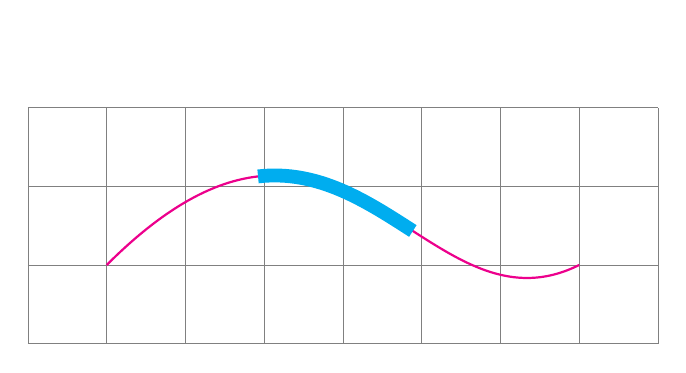
\begin{tikzpicture}
  \draw[help lines] (-1,-1) grid (7,2);
  \coordinate (P0) at (0,0);
  \coordinate (P1) at (3,3);
  \coordinate (P2) at (4,-1);
  \coordinate (P3) at (6,0);
  \draw[thick,magenta] (P0) .. controls (P1) and (P2) .. (P3);
  \drawbeziersub[line width=5pt,cyan]{P0}{P1}{P2}{P3}{0.25}{0.6}
\end{tikzpicture}
\end{document}
